\documentclass[border=10pt]{standalone}

\usepackage{tikz}
\usepackage{tikzsymbols}
\usetikzlibrary{calc,patterns,shapes.geometric}

\def\centerarc[#1](#2)(#3:#4:#5){\draw[#1] ($(#2)+({#5*cos(#3)},{#5*sin(#3)})$) arc (#3:#4:#5);}

\begin{document}
	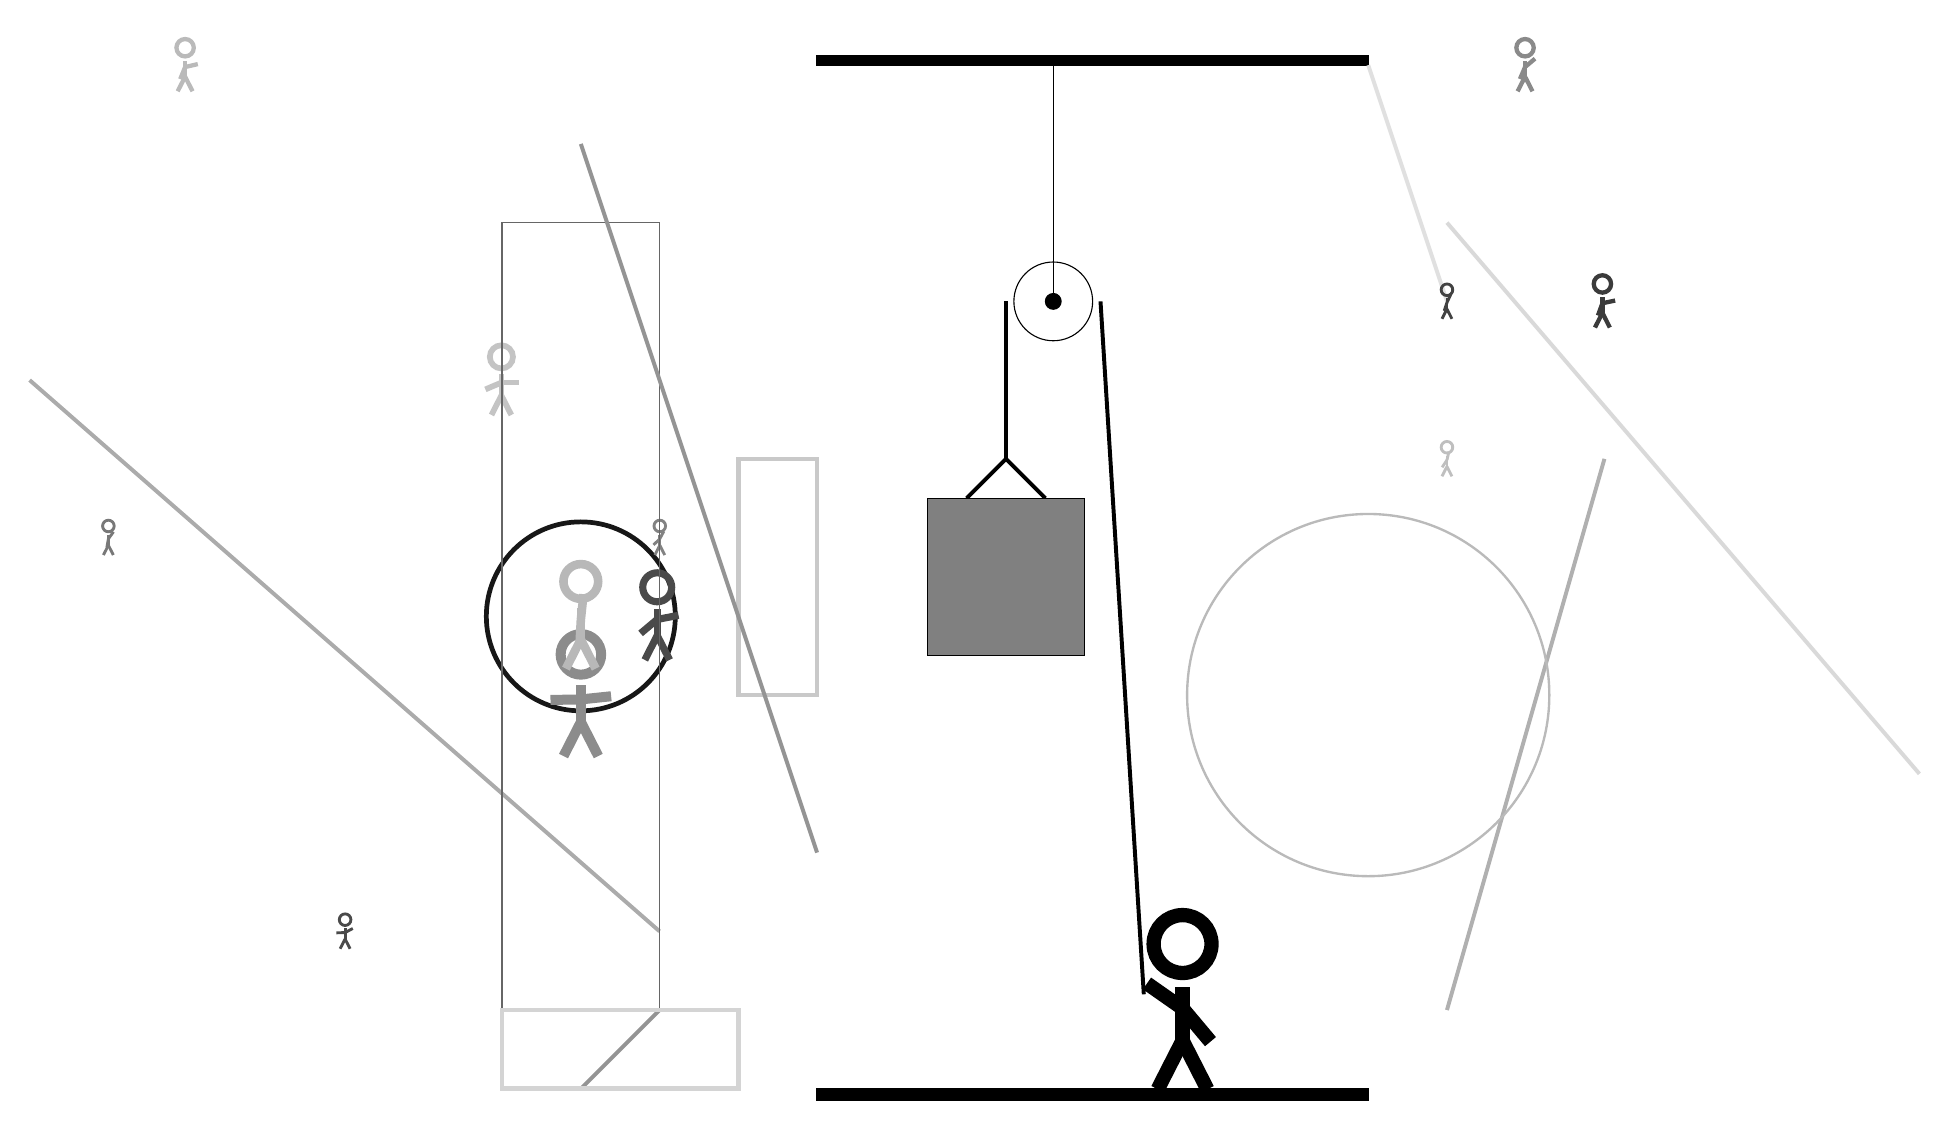
\begin{tikzpicture}
		%%%%% START %%%%%
		
		\draw[fill=black] (-2, 10) rectangle (5, 10.125);
		
		\draw[line width=0.5mm, color=black!42](-4, -2) -- (-5, -3);
		
		\draw[line width=0.5mm, color=black!15](6, 8) -- (12, 1);
		\draw[line width=0.6mm, color=black!21] (-3, 5) rectangle (-2, 2);
		\node[line width=0.7mm, color=black!53] at (-11, 4) {\Strichmaxerl[2][80][54]};
		\draw [line width=0.6mm, color=black!91](-5, 3) circle (1.2);
		
		\node[line width=0.3mm, color=black!45] at (-5, 2) {\Strichmaxerl[7][1][6]};
		\node[line width=0.3mm, color=black!25] at (6, 5) {\Strichmaxerl[2][56][77]};
		\draw[line width=0.5mm, color=black!31](6, -2) -- (8, 5);
		\draw[line width=0.5mm, color=black!33](-4, -1) -- (-12, 6);
		\node[line width=0.2mm, color=black!71] at (-4, 3) {\Strichmaxerl[5][40][11]};
		
		\draw[line width=0.5mm, color=black!12](6, 7) -- (5, 10);
		\node[line width=0.7mm, color=black!23] at (-6, 6) {\Strichmaxerl[4][23][0]};
		\node[line width=0.3mm, color=black!49] at (-4, 4) {\Strichmaxerl[2][44][62]};
		\node[line width=0.3mm, color=black!77] at (8, 7) {\Strichmaxerl[3][70][12]};
		\node[line width=0.3mm, color=black!74] at (6, 7) {\Strichmaxerl[2][71][65]};
		\draw[line width=0.2mm, color=black!60] (-4, -2) rectangle (-6, 8);
		\node[line width=0.4mm, color=black!46] at (7, 10) {\Strichmaxerl[3][67][40]};
		\node[line width=0.4mm, color=black!28] at (-5, 3) {\Strichmaxerl[6][87][84]};
		\node[line width=0.6mm, color=black!27] at (-10, 10) {\Strichmaxerl[3][68][13]};
		\draw [line width=0.3mm, color=black!27](5, 2) circle (2.3);
		\node[line width=0.3mm, color=black!71] at (-8, -1) {\Strichmaxerl[2][2][28]};
		\draw[line width=0.6mm, color=black!17] (-3, -3) rectangle (-6, -2);
		
		\draw[line width=0.5mm, color=black!42](-2, 0) -- (-5, 9);
		
		\draw (1, 7) circle (0.5);
		\draw[fill=black] (1, 7) circle (0.1);
		\draw (1, 10) -- (1, 7);
		
		\draw[line width=0.5mm] (-0.1, 4.5) -- (0.4, 5.0) -- (0.9, 4.5);
		\draw[fill=black!50] (-0.6, 4.5) rectangle (1.4, 2.5);
		
		\draw[line width=0.5mm] (0.4, 7) -- (0.4, 5.0);
		\centerarc[line width=0.5mm](1, 7)(0:180:0.6);
		\draw[line width=0.5mm](1.6, 7) -- (2.15, -1.8);
		
		\node at (2.6, -1.9) {\Strichmaxerl[10][-35][-50]};
		
		\draw[fill=black] (-2, -3) rectangle (5, -3.15);
		
		%%%%% END %%%%%
	\end{tikzpicture}
\end{document}